
\section{Introduction}
% intro
Machine learning (ML) has many applications in experimental particle physics, including event identification and reconstruction.
One aspect of reconstruction is calorimeter cluster calibration, which is the focus of this thesis.
This chapter introduces some background on the ML methods used, which are discussed in the following chapters. %(Check this source for more info and source).

Before discussing ML, it is important to introduce Artificial intelligence (AI).
AI is the process of training computers to imitate how the human brain learns and solves problems.
%An AI computer program, software, could be simple as a chess game or complex as one that can predict the RNA structure of a virus to help develop vaccinee. %source1.
AI-powered software can range from simple applications, such as a chess program, to complex systems capable of predicting the RNA structure of a virus to aid in vaccine development.
There are different types of AI, as shown in Fig.~\ref{fig:ML_diagram}, and ML is a subset of AI and deep learning (DL) is a subset of ML.
%To understand the difference between ML and DL, ML is of AI where it needs a human intervene to improve its learning and DL where computers learn from its own past mistakes. %(Source for more info about deep learning.)
ML requires human intervention to improve its learning, whereas DL enables computers to refine their learning from its own past mistakes.

\begin{figure}[t!]
\centering
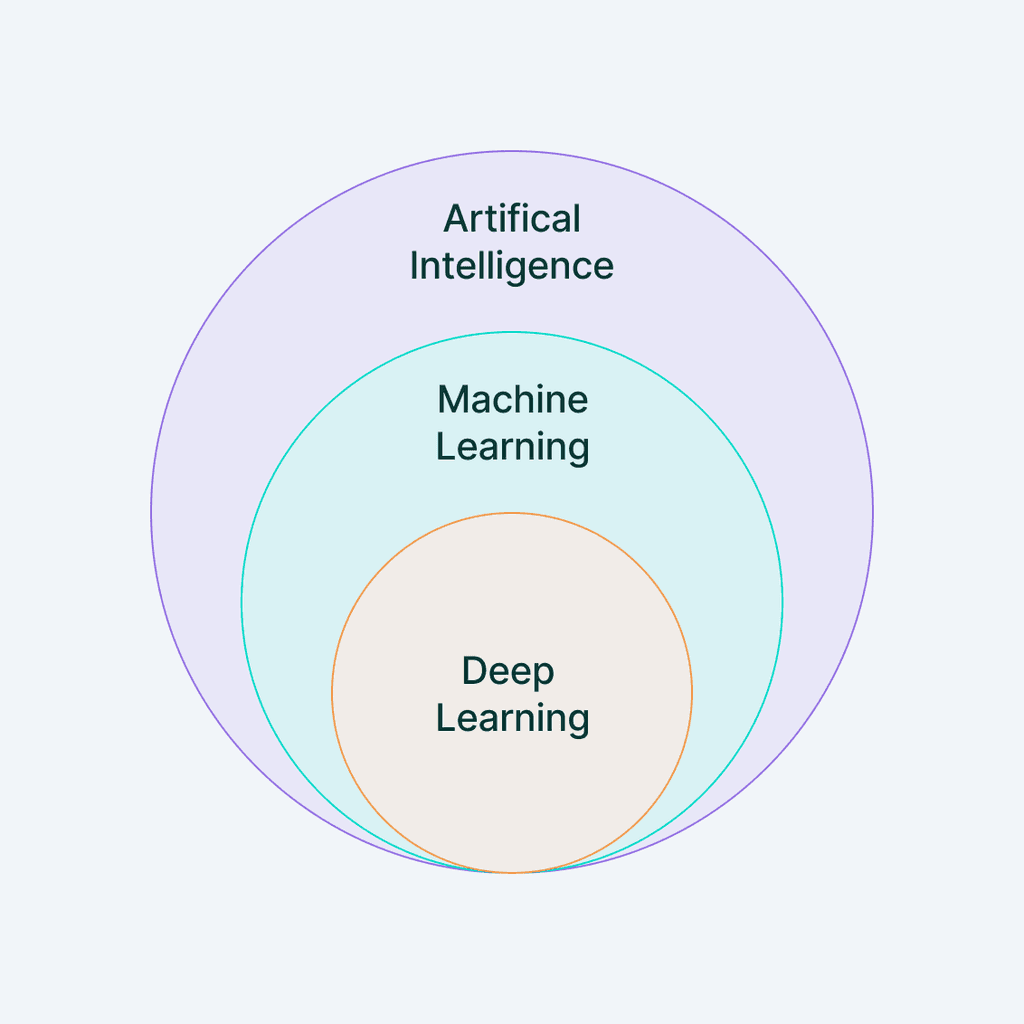
\includegraphics[width=0.99\textwidth]{figures/ML_diagram.png}
\caption[ML and AI]{Figure source~\cite{SMtable}.}
\label{fig:ML_diagram}
\end{figure}

In ML there are few concepts to be familiar with, such as Al algorithm and ML model.
% (fix me- these concepts will be used a lot in the next chapters).
An AI algorithm is a set of programmed instructions that tells the computer how to learn and operate on its own %(source2)
to solve a problem or to do a task.
ML models are computer programs used to recognize patterns in data (classification) or make predictions (regression).
ML models are created using ML algorithms that undergo a training process with a data.
In this process, the algorithm is adjusted and optimized to improve its ability to handle a specific task, resulting in a trained ML model.
%to modified the algorithm to be better at manage the specific task and becomes a ML model. % Source3

ML algorithms could be categorized into three main groups depending on type of data used in the training process: supervised learning, unsupervised learning, reinforcement learning, as seen in figure related. % (source)
Data could be either labeled or unlabeled.
Labeled data is any data the has an attribute or category assigned to, for example, the price of a product or the height of a human.
For ML algorithms and model implementation various python-based libraries, such as schitkit-learn, TensorFlow, and keras are used.
The rest of this chapter will describe the commonly used ML algorithms in HEP: %source
boosted decision trees and neural networks.

\section{Boosted Decision Tree}
A decision trees (DT), as seen in the related figure, is a type of algorithm that looks like an upside-down tree that starts with a root at the top, and then branches out to leaves.
A DT has different level of nodes: Root node is a top most node and it represent the entire message of the decision.
Decision node is a node where the prior node branches into two or more.
Leaf node is the last node in DT and represents the outcome or prediction of the decision process.
DTs are supervised learning algorithms that can be used to make classification and regression models.
This thesis deals with regression problems.

In each node of DT, the split is chosen to maximize the information gain (difference between in entropy before and after the potential split), in other words, minimizing the entropy.
Entropy is maximum for 50/50 split and minimum for 1/0 split, \ie contains only one class.
The spilt is created recursively (iteratively), with each split chosen to maximize the information gain.
This process continues until a stopping condition is met, such as reaching a maximum tree depth or when no further information gain is possible.

In boosted decision trees (BDT), DT uses a boosting technique that iteratively works to improve the weak trees by combining them. %KenH (KenH belieave that's what Noorah meant) more, tree, that will correct the error of the previous one.
%How this works, the new tree will be trained on the samples that were misclassified by the previous tree which gradually will refine the overall accuracy (fix me).
Each new tree is trained on the samples misclassified by the previous tree, gradually refining the overall accuracy of the model.
In BDT, the final prediction is the weighted average of all models (trees) with more weight given to those with higher accuracy.
There are different ways to iteratively adding learners, %to minimize a loss function
with some of the common ones being Adaboost (adaptive boosting), Gradient Boosting, XGBoost which will be used later for ECAL cluster calibration.

\section{Neural Network}
Neural Networks (NN), also known as Artificial Neural Networks (ANN), are called so, because of the way how they mimic the neurons in the brain sending signals to each other.
%They are one of the most used ML algorithms (in particle physics).
They are among the most widely used ML algorithms in particle physics.
The simplest NN contains an input layer, output layer, and one hidden layer, %each containing number of neurons that are connected.
with each layer containing a number of interconnected neurons.
%NN’s are the backbone of DL algorithms if they have more one hidden layer. %(insert picture of a simple NN vs DL with multiple layers)
When a neural network has more than one hidden layer, it forms the foundation of DL algorithms.

NN, like other DL algorithms, rely on the training data to learn and improve its accuracy overtime without human intervention.
As mentioned before each layer have multiple neurons, and each one of those neurons
can be thought of as a linear regression model with its own activation function. Each neuron processes input data, applies weights and biases, and produces an output.
%could think of it as its one linear regression model, activation function) contains input data, weights, bias, and output. (fix me)

All inputs are then multiplied by their respective weights (which helps determine the importance of each input variable) and then summed together.
The resulting sum, along with a bias, is passed through an activation function (\eg{}, ReLU, sigmoid).
If the output exceeds a certain threshold, the neuron is activated, and the data is passed to the next layer in the network.
%Afterward the output (with bias) is passed through the activation function (example of activation function?) if the output exceeds a given threshold, it activates the node and passing data to the next layer in the network.
This results in the output of one node becoming in the input of the next node.
This process of passing data from one layer to the next layer defines this NN as a feedback network.
%The goal is minimizing errors (cost/loss function, example) to insure the fitting of the model.
The primary goal of training the network is to minimize errors (using a cost or loss function, such as mean squared error or cross-entropy), ensuring that the model fits the data accurately.

As the model learns, it adjusts its weights and biases to reduce the error. This process continues until the network reaches a local minimum of the loss function, typically achieved through an optimization technique such as gradient descent.
%As the model adjusts its weight and bias.
%Until reaches a local minimum (mention gradient decent).
